\section{Текст программы}

\lstinputlisting[language=Matlab]{../../src/lab02.m}


\section{Результат работы программы}
\begin{align*}
	\hat\mu(\vec x_n) &= -4.76; \\
	S^2(\vec x_n)     &= 0.81;  \\
	\underline{\mu}(\vec x_n) &= -4.89; \\
	\overline{\mu}(\vec x_n) &= -4.62; \\
	\underline{\sigma^2}(\vec x_n) &= 0.66; \\
	\overline{\sigma^2}(\vec x_n) &= 1.02; \\
\end{align*}

\pagebreak
\section{Графики}
\begin{figure}[h!]
	\centering
	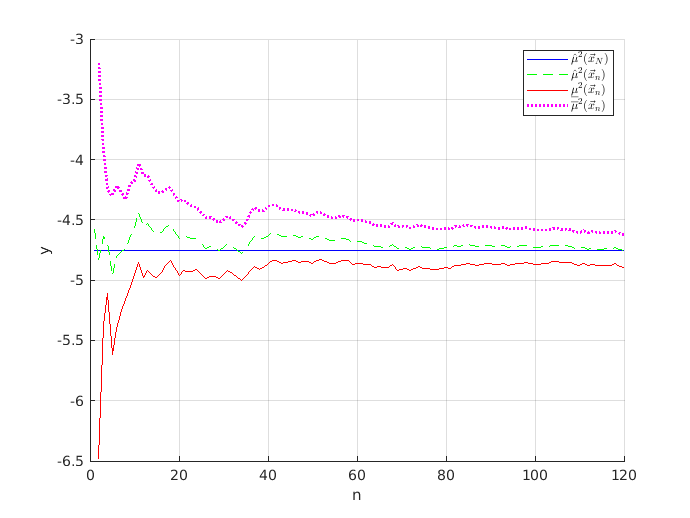
\includegraphics{../img/figure21}
	\caption{График для $\mu$}
\end{figure}

\begin{figure}[h]
	\centering
	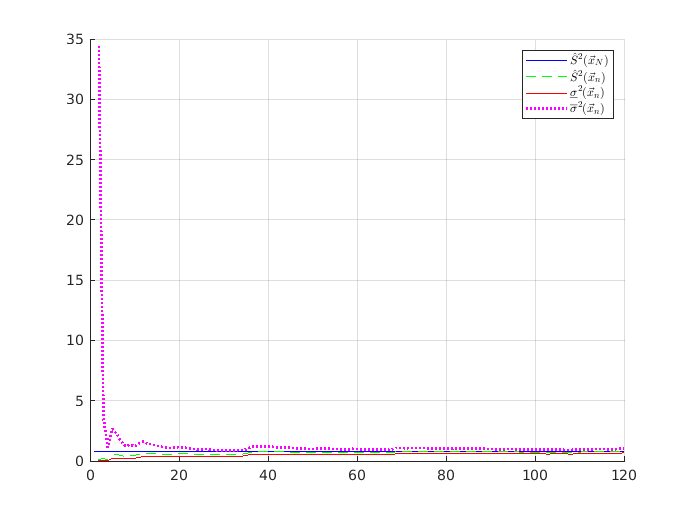
\includegraphics{../img/figure22}
	\caption{График для $\sigma$}
\end{figure}